\documentclass[10pt,a4paper]{article}
\usepackage[margin=1.6cm]{geometry}
\usepackage{lmodern}
\usepackage{graphicx}
\usepackage{booktabs}
\usepackage{siunitx}
\usepackage{xcolor}
\usepackage{enumitem}
\usepackage[hidelinks]{hyperref}
\usepackage{multicol}
\usepackage{tabularx}
\setlength{\parindent}{0pt}\setlength{\parskip}{4pt}
\pagestyle{empty}
\definecolor{acc}{HTML}{C0392B}
\newcommand{\hl}[1]{\textcolor{acc}{\textbf{#1}}}
\begin{document}
{\LARGE\textbf{FlexTome}}\quad{\large a 3D-printed, flexure-pivot rocking microtome with a differential-screw feed}\\[2pt]
{\small Design study, revision 2. Companion to the full report (\emph{flextome\_paper.pdf}). All performance numbers are model predictions; the machine has not yet been built.}

\vspace{4pt}\hrule\vspace{6pt}

\begin{minipage}[t]{0.56\linewidth}\vspace{0pt}
\textbf{The problem.} Diagnostic histology needs 3--\SI{5}{\micro\metre} paraffin sections. A new manual rotary microtome costs US\$9\,000--22\,700; the thinnest published open-source sectioning device cuts at $\geq$\SI{50}{\micro\metre}. Much of sub-Saharan Africa has about one pathologist per million people, and the microtome is one of the few items in the diagnostic chain with no low-cost substitute.

\textbf{The idea.} Put the micrometre-scale motion entirely in steel and let the printed plastic do only millimetre-scale jobs:
\begin{enumerate}[nosep,leftmargin=1.2em]
\item \textbf{Cross-strip flexure pivot}: three \SI{0.20}{\milli\metre} spring-steel feeler-gauge strips carry the \SI{125}{\milli\metre} arm; no sliding or rolling joint, no backlash.
\item \textbf{Differential screw from two standard threads}: M8$\times$1.25 against M8$\times$1.0 gives \SI{0.25}{\milli\metre} per turn; a 50-tooth printed ratchet divides that into \hl{\SI{5}{\micro\metre} steps}, selectable 5--\SI{30}{\micro\metre}.
\item \textbf{Printed parallelogram flexure stage} carries the blade and is spring-preloaded onto the screw, so the feed has no backlash either.
\end{enumerate}
A crank-rocker turns one handwheel revolution into one \SI{54}{\milli\metre} stroke and one section; the arm itself advances the ratchet at the top of each stroke.

\textbf{Strongest result.} With every element of the force path drawn, connected and either calculated or finite-element modelled, the loop between blade edge and block face has a stiffness of \hl{\SI{0.83}{\newton\per\micro\metre}}, and a Monte-Carlo budget predicts sections of \hl{$5.0\pm0.7$\,\si{\micro\metre}} (1~s.d.; 90\,\% interval 3.8--\SI{6.2}{\micro\metre}) at the \SI{5}{\micro\metre} setting, at a bill of materials of \hl{US\$61.97}. For context, a 154-site survey found more than two-thirds of sections from commercial microtomes outside $\pm10\,\%$ of the dial setting.
\end{minipage}\hfill
\begin{minipage}[t]{0.42\linewidth}\vspace{0pt}
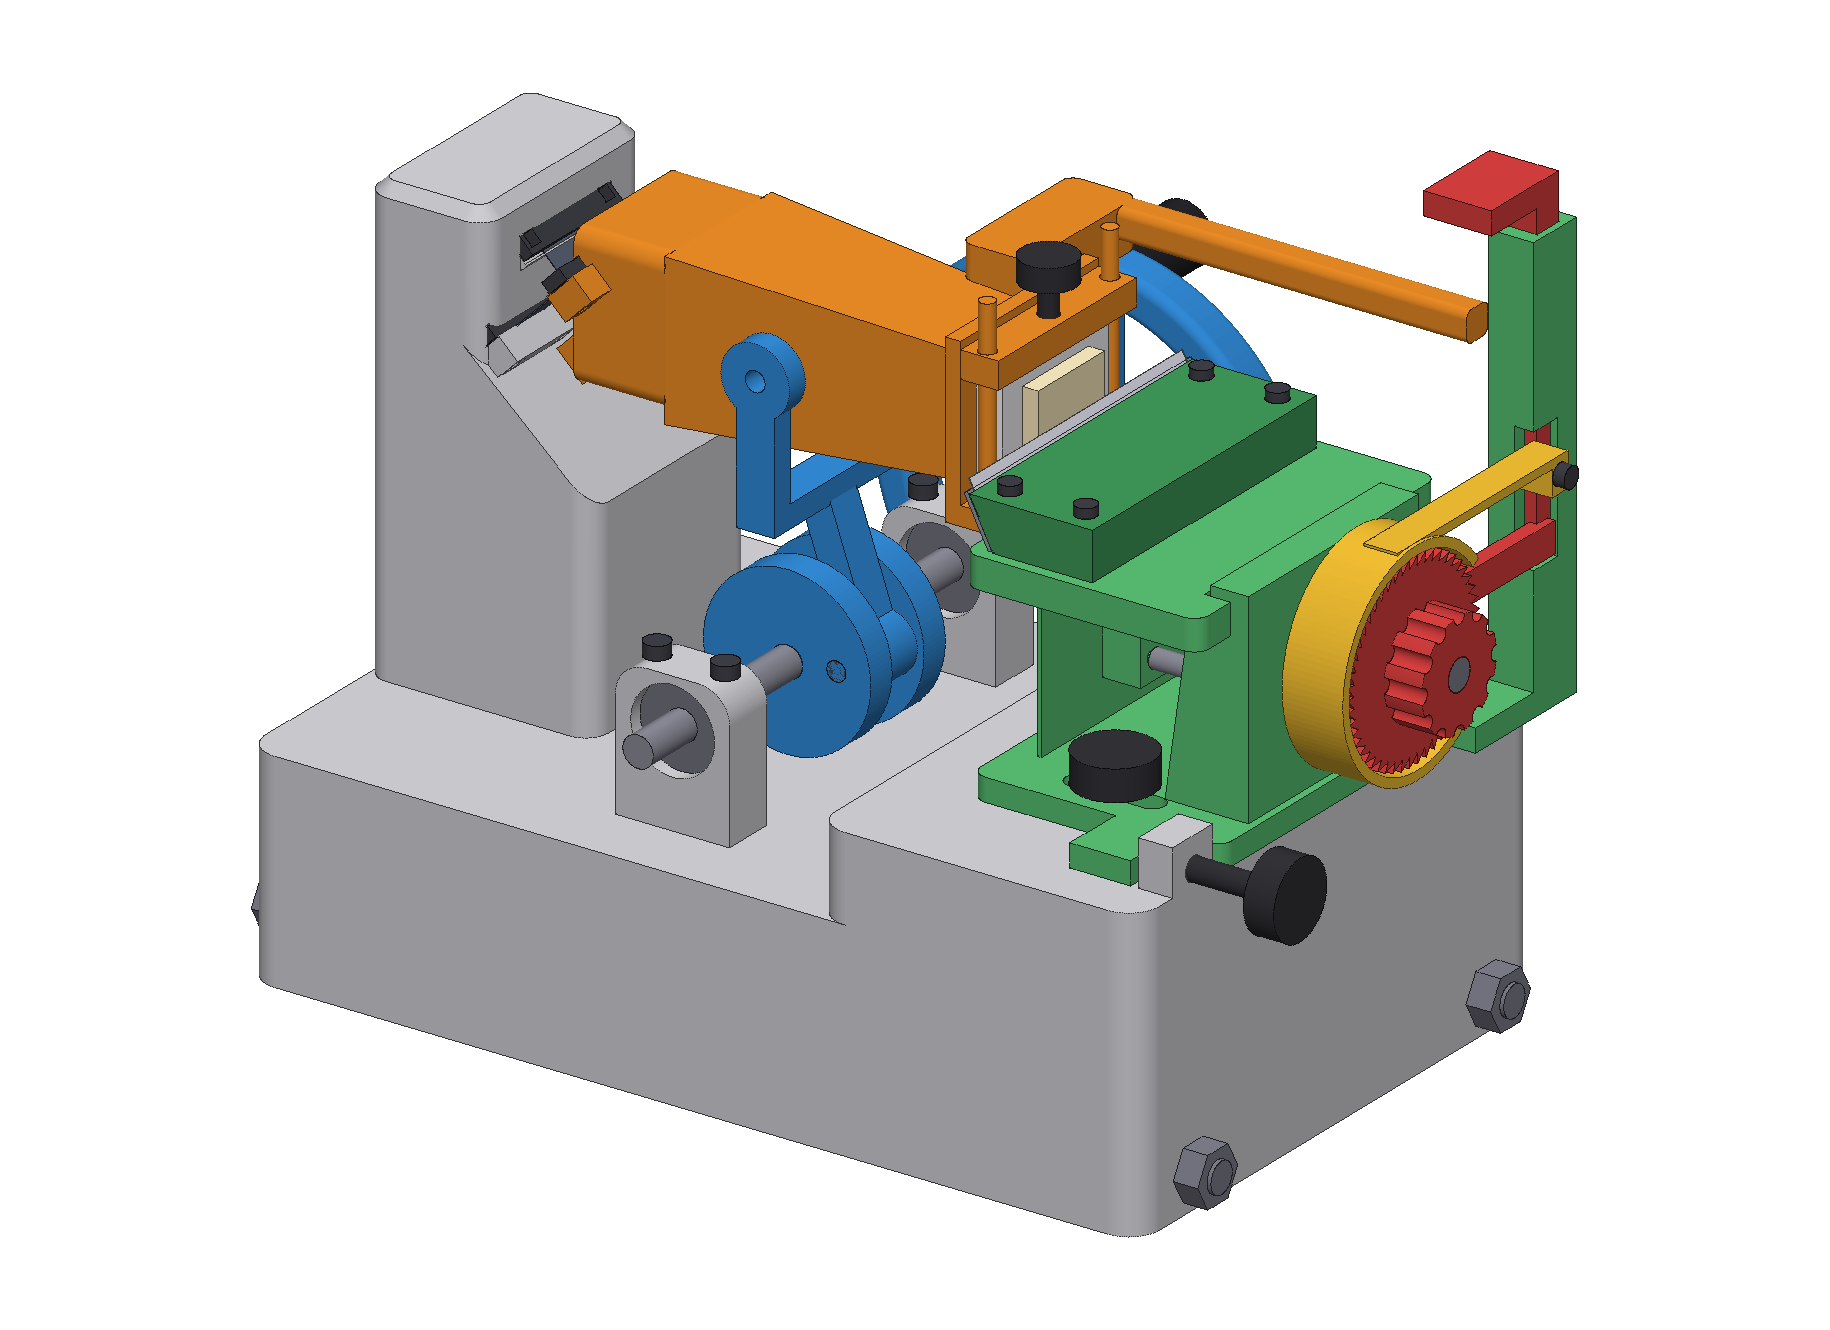
\includegraphics[width=\linewidth]{figures/fig_render_iso_right.png}
{\footnotesize Revision-2 assembly: 16 printed part types (20 pieces, \SI{1.4}{\litre} PLA) plus hardware-store steel. Frame $235\times150\times\SI{173}{\milli\metre}$, one print on a \SI{235}{\milli\metre} bed. Envelope $275\times210\times\SI{202}{\milli\metre}$.}
\end{minipage}

\vspace{6pt}
\begin{minipage}[t]{0.49\linewidth}\vspace{0pt}
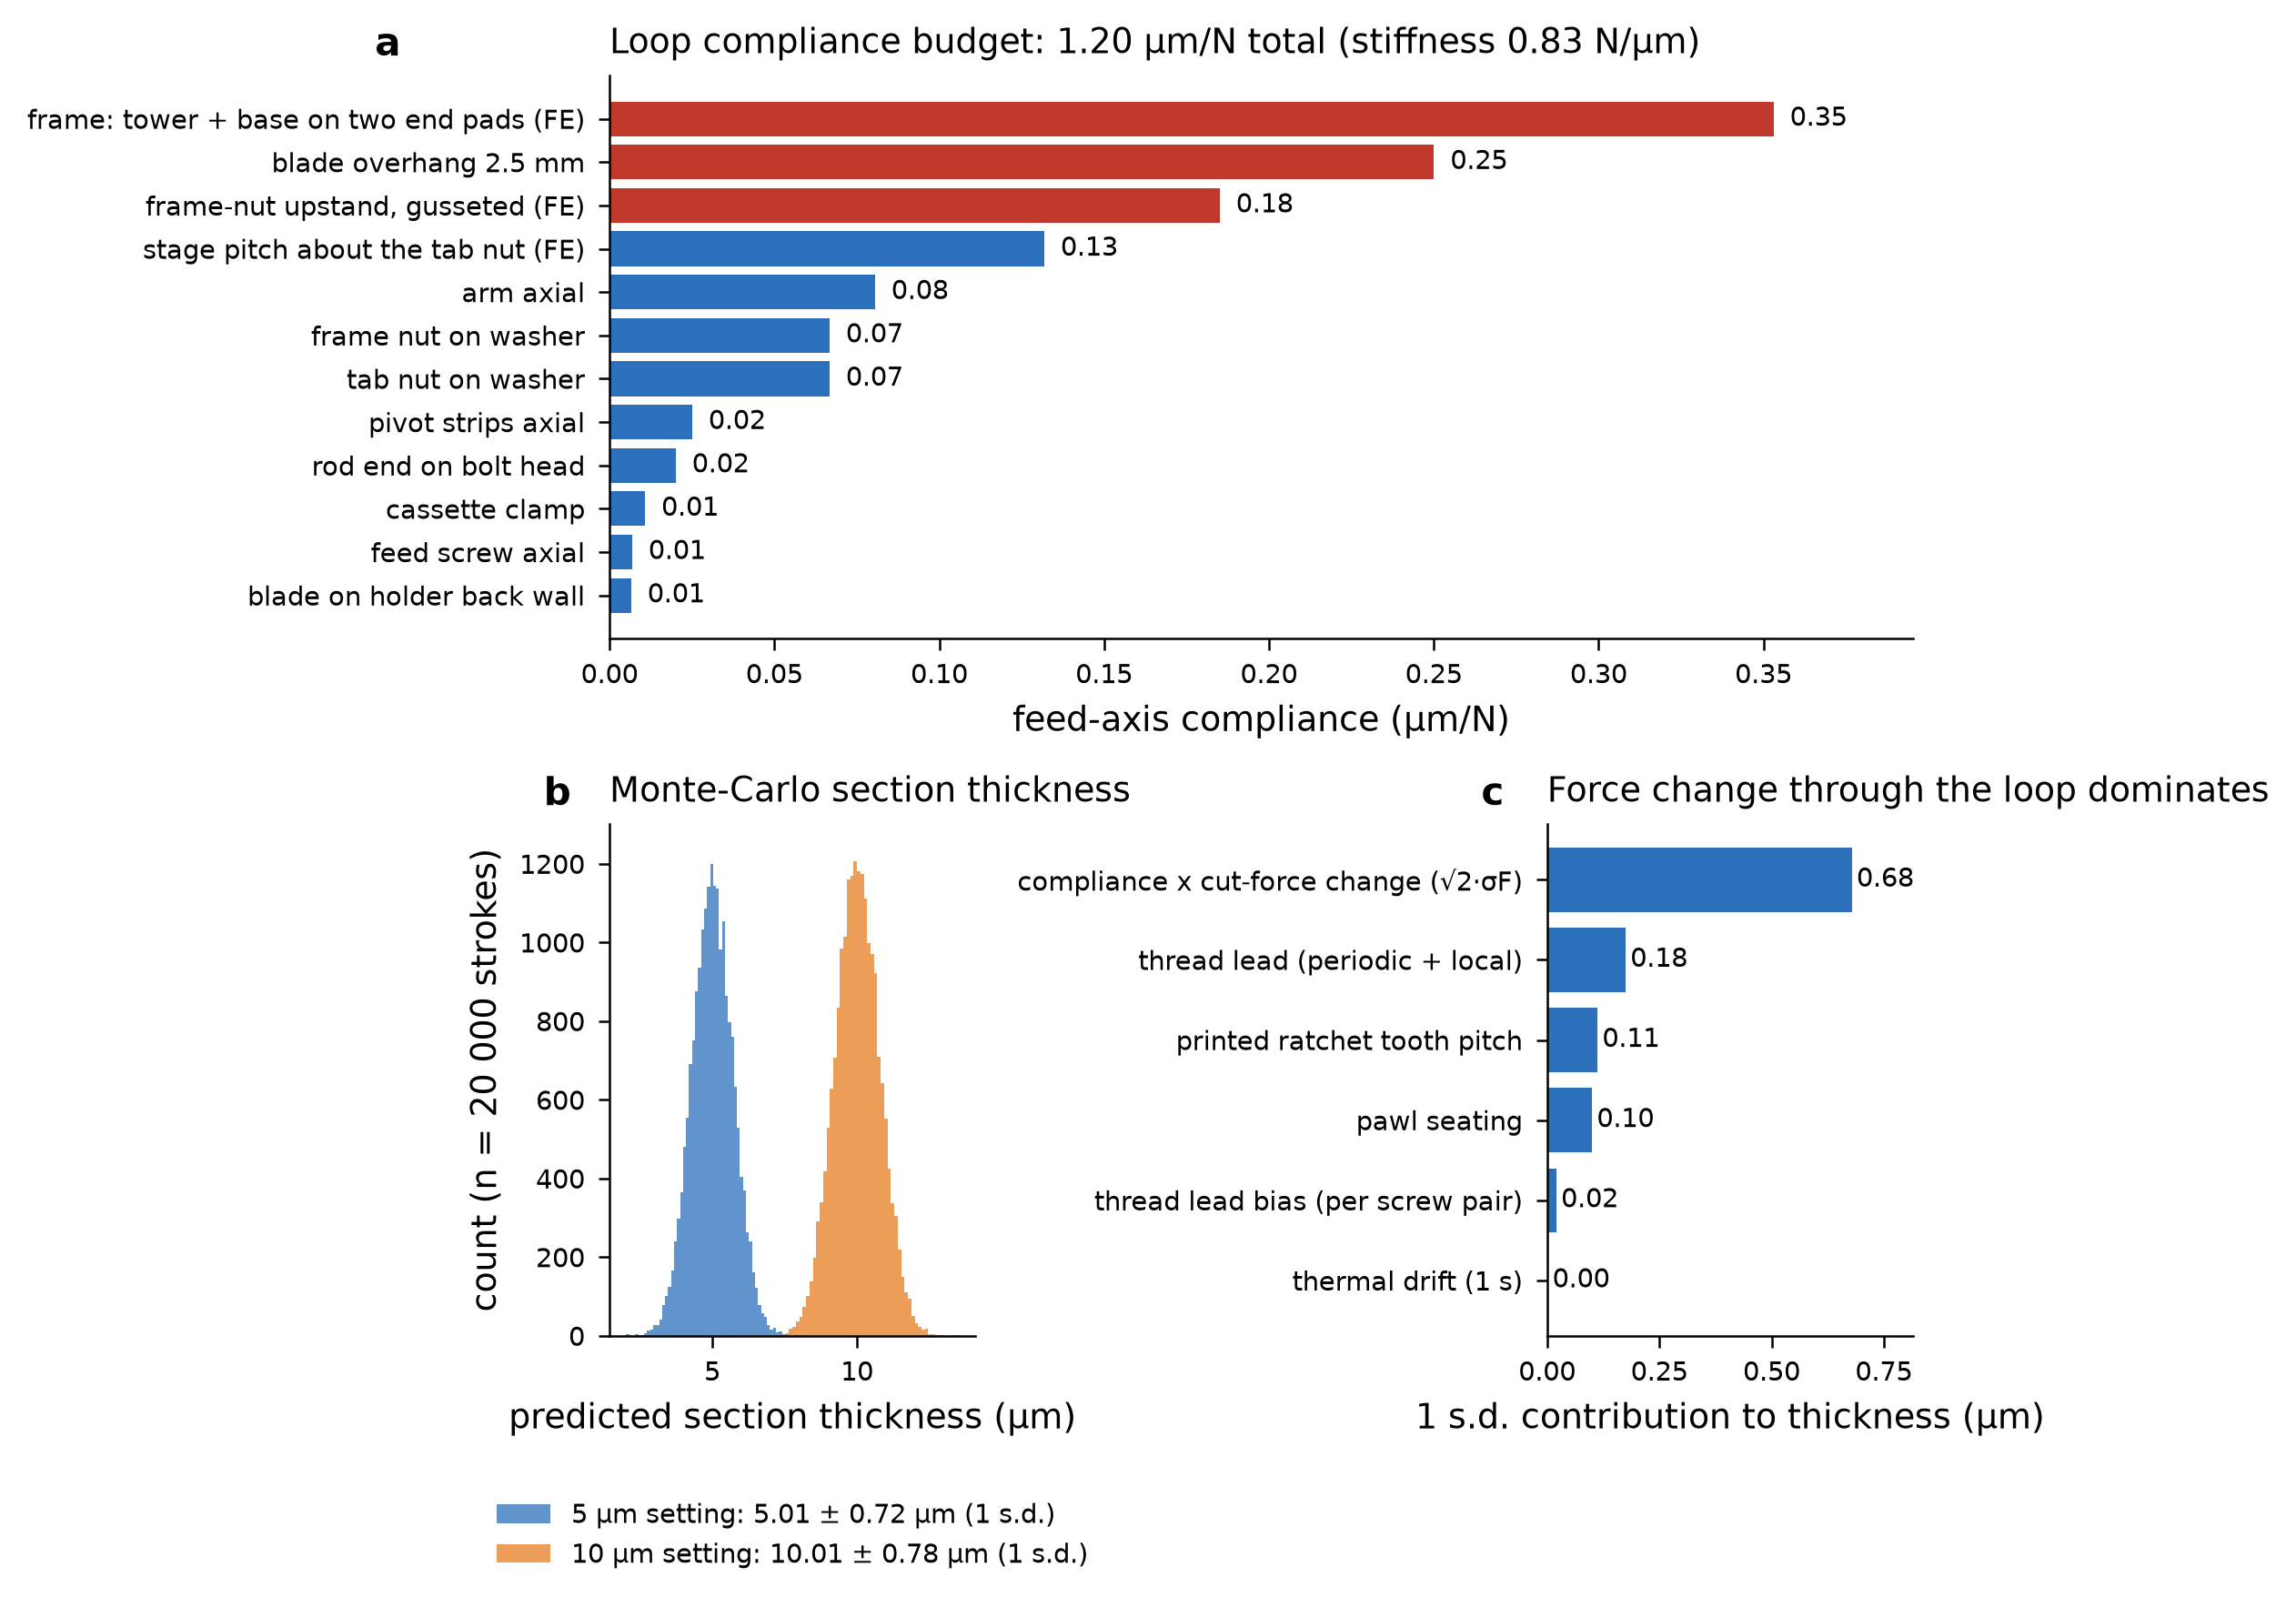
\includegraphics[width=\linewidth]{figures/fig3_error_budget.png}
{\footnotesize Where the compliance is (a) and what sets the thickness scatter (b, c). Stroke-to-stroke change in cutting force acting through the loop dominates; the steel feed chain contributes little.}
\end{minipage}\hfill
\begin{minipage}[t]{0.49\linewidth}\vspace{0pt}
\textbf{Key numbers}\\[-8pt]
\begin{center}\small
\begin{tabularx}{\linewidth}{@{}Xr@{}}
\toprule
Stroke / arm swing & \SI{54}{\milli\metre} / $\pm$\ang{12.5} \\
Feed per turn / per ratchet tooth & \SI{0.25}{\milli\metre} / \SI{5.0}{\micro\metre} \\
Loop compliance (stiffness) & \SI{1.20}{\micro\metre\per\newton} (\SI{0.83}{\newton\per\micro\metre}) \\
Predicted section, \SI{5}{\micro\metre} setting & $5.01\pm0.72$\,\si{\micro\metre} \\
Predicted section, \SI{10}{\micro\metre} setting & $10.01\pm0.78$\,\si{\micro\metre} \\
Thread-lead bias (per machine) & within $\pm0.7\,\%$ \\
Pivot strip stress at full swing & \SI{218}{\mega\pascal} (fatigue SF 2.1) \\
First structural mode & \SI{357}{\hertz} (cut excites $<$\SI{9}{\hertz}) \\
Bill of materials & US\$61.97 \\
\bottomrule
\end{tabularx}
\end{center}
\textbf{What the external review changed.} An independent check of revision~1 found that its budget did not match its CAD: the feed-screw upstand was disconnected and only \SI{6}{\milli\metre} thick (\SI{7.3}{\micro\metre\per\newton} on its own), the blade was held on two screw tips, the coupler was \SI{0.7}{\milli\metre} thick, and the Monte-Carlo under-counted the force term by $\sqrt2$. Revision~2 gussets and connects the upstand (\SI{0.19}{\micro\metre\per\newton}), gives the blade a full-width back wall, makes the coupler's axial path steel-on-steel, adds preload springs and washers, and re-derives every error as a stroke-to-stroke difference. Had revision~1 been built, the model says it would have cut $5\pm4.8$\,\si{\micro\metre}.
\end{minipage}

\newpage
\begin{center}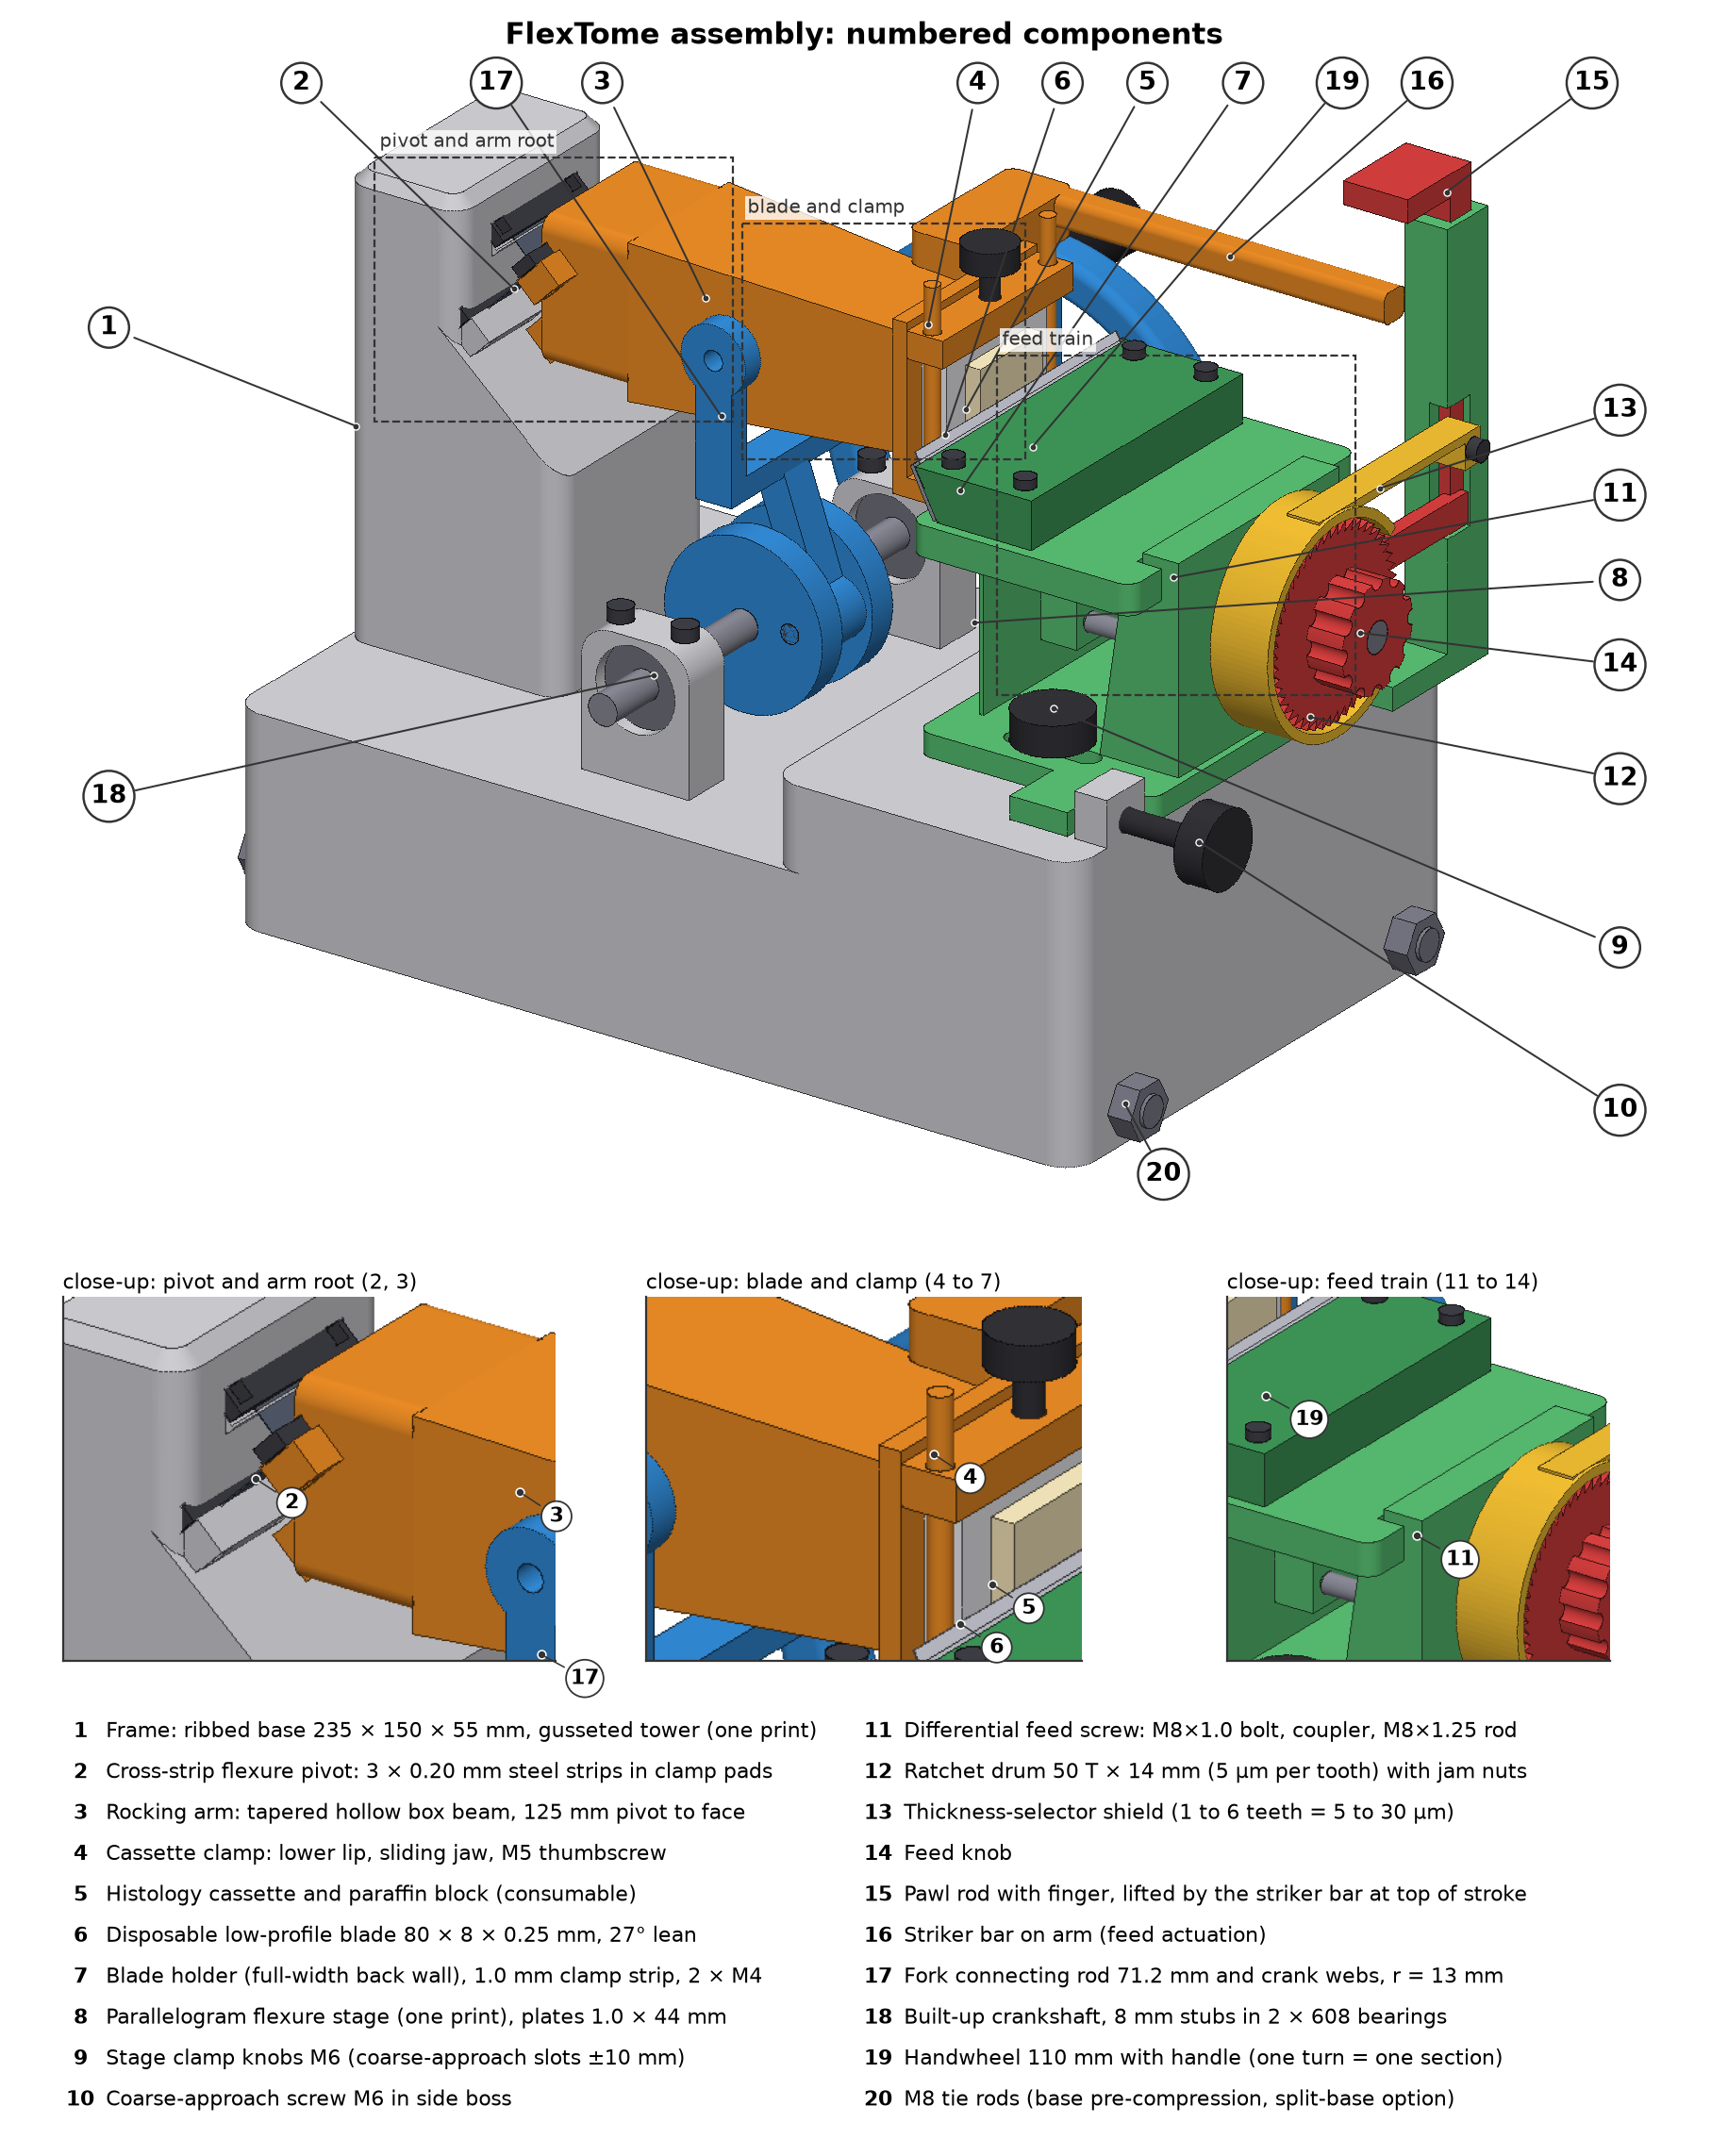
\includegraphics[height=0.62\textheight]{figures/fig1_assembly_callouts.png}\end{center}
\vspace{2pt}
\begin{minipage}[t]{0.49\linewidth}\vspace{0pt}
\textbf{How it works in one sentence each}
\begin{itemize}[nosep,leftmargin=1.2em]
\item \emph{Drive}: handwheel $\rightarrow$ two-web crankshaft ($r=\SI{13}{\milli\metre}$) $\rightarrow$ fork rod $\rightarrow$ arm joint at \SI{60}{\milli\metre}; $\sin\theta_{\max}=13/60$.
\item \emph{Cut}: blade leans \ang{27}; clearance \ang{9.5}, rake \ang{45.5}; the face is trimmed to the \SI{125}{\milli\metre} arc once, then every section is the difference of two identical arcs.
\item \emph{Feed}: $\Delta x = (1.25-1.00)/50 = \SI{5}{\micro\metre}$ per tooth; the striker bar lifts the pawl past $\theta\approx\ang{6}$, the pawl indexes the drum on the way down, before the face reaches the edge.
\item \emph{Why it can work in plastic}: only the force path from edge to block face sets thickness; a steady cutting force is trimmed into the block, only its stroke-to-stroke change matters.
\end{itemize}
\end{minipage}\hfill
\begin{minipage}[t]{0.49\linewidth}\vspace{0pt}
\textbf{What is still assumed, and what to measure first}
\begin{itemize}[nosep,leftmargin=1.2em]
\item The feed-axis cutting force ($2\pm0.4$\,N per stroke) is an assumption bracketed by a fracture model (0.23--\SI{0.86}{\newton}); no absolute paraffin value exists in the literature. Scatter scales almost linearly with it.
\item Nut bedding on washers (\SI{1.5e7}{\newton\per\metre}) and the PLA creep limit (\SI{15}{\mega\pascal}) are allowances, not measurements.
\item Levers if a build cuts thick-thin: back-wall overhang \SI{2.0}{\milli\metre}, base shimmed to full contact, brass inserts: together \SI{0.90}{\micro\metre\per\newton} and \SI{0.56}{\micro\metre}.
\item Build-and-measure protocol (in the report): loop stiffness with a \SI{2}{\newton} load and a dial gauge, feed per tooth over 50 teeth, then 100 consecutive \SI{5}{\micro\metre} sections measured by profilometry or weighing.
\end{itemize}
\textbf{Repository}: CadQuery source, STEP, 35 STLs, FE and Monte-Carlo code, interference and mesh-connectivity audit, BOM, LaTeX sources.
\end{minipage}
\end{document}
